%=========================================================================
% fig-xpc-isa.tex
%=========================================================================

%\begin{figure}

  \centering
  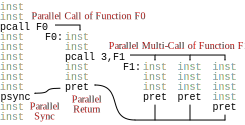
\includegraphics[width=0.9\tw]{xpc-isa.svg.pdf}

  \caption{\textbf{XPC Instruction Set Overview --} Parallel calls and
    parallel multi-calls (\TT{pcall}) encode opportunities for parallel
    execution, which the architecture may (or may not) choose to exploit.
    Parallel synchronization points (\TT{psync}) require all child
    parallel calls to complete before continuing. All parallel returns
    (\TT{pret}) are implicitly synchronization points.}

  \label{fig-xpc-isa}

%\end{figure}

